% document style header
\documentclass[a4paper, 12pt]{config/homework}

% import default packages
\usepackage{config/defpackages}
% import custom math commands
\usepackage{config/domath}
\usepackage{pdfpages}

% end preamble
\begin{document}

% document title
\noindent
\begin{tabularx}{\textwidth}{>{\centering\arraybackslash}X>{\centering\arraybackslash}X>{\centering\arraybackslash}X}
Calvin Sprouse & PHYS489 A2 & 2024 January 23\\
\midrule
\end{tabularx}

% reflection prompt
% Select and write a reflection on a graded lab report from one of the upper division physics lab classes that you think best demonstrates the learning outcome of applying experimental methods. Applying experimental methods generally involves applying a multiple component apparatus and/or multiple instruments; applying physical models in the experimental context; developing and applying methods and procedures to achieve an experimental goal; and analyzing, interpreting, and reporting results. Upper division physics lab classes include PHYS 303, 306, 323, 331, 333, 334, 433, 454.

% Scan your selected artifact(s) and combine these into a single PDF document.
% Prepare a 1/2 page reflection on how the artifact demonstrates your progress to meeting this goal.
% Upload both pdf documents to Canvas by 11:59pm Friday, January 26.

% reflection
The artifact I selected is my final lab report for PHYS333 Experimental Physics on the Franck Hertz experiment.

% insert artifact page
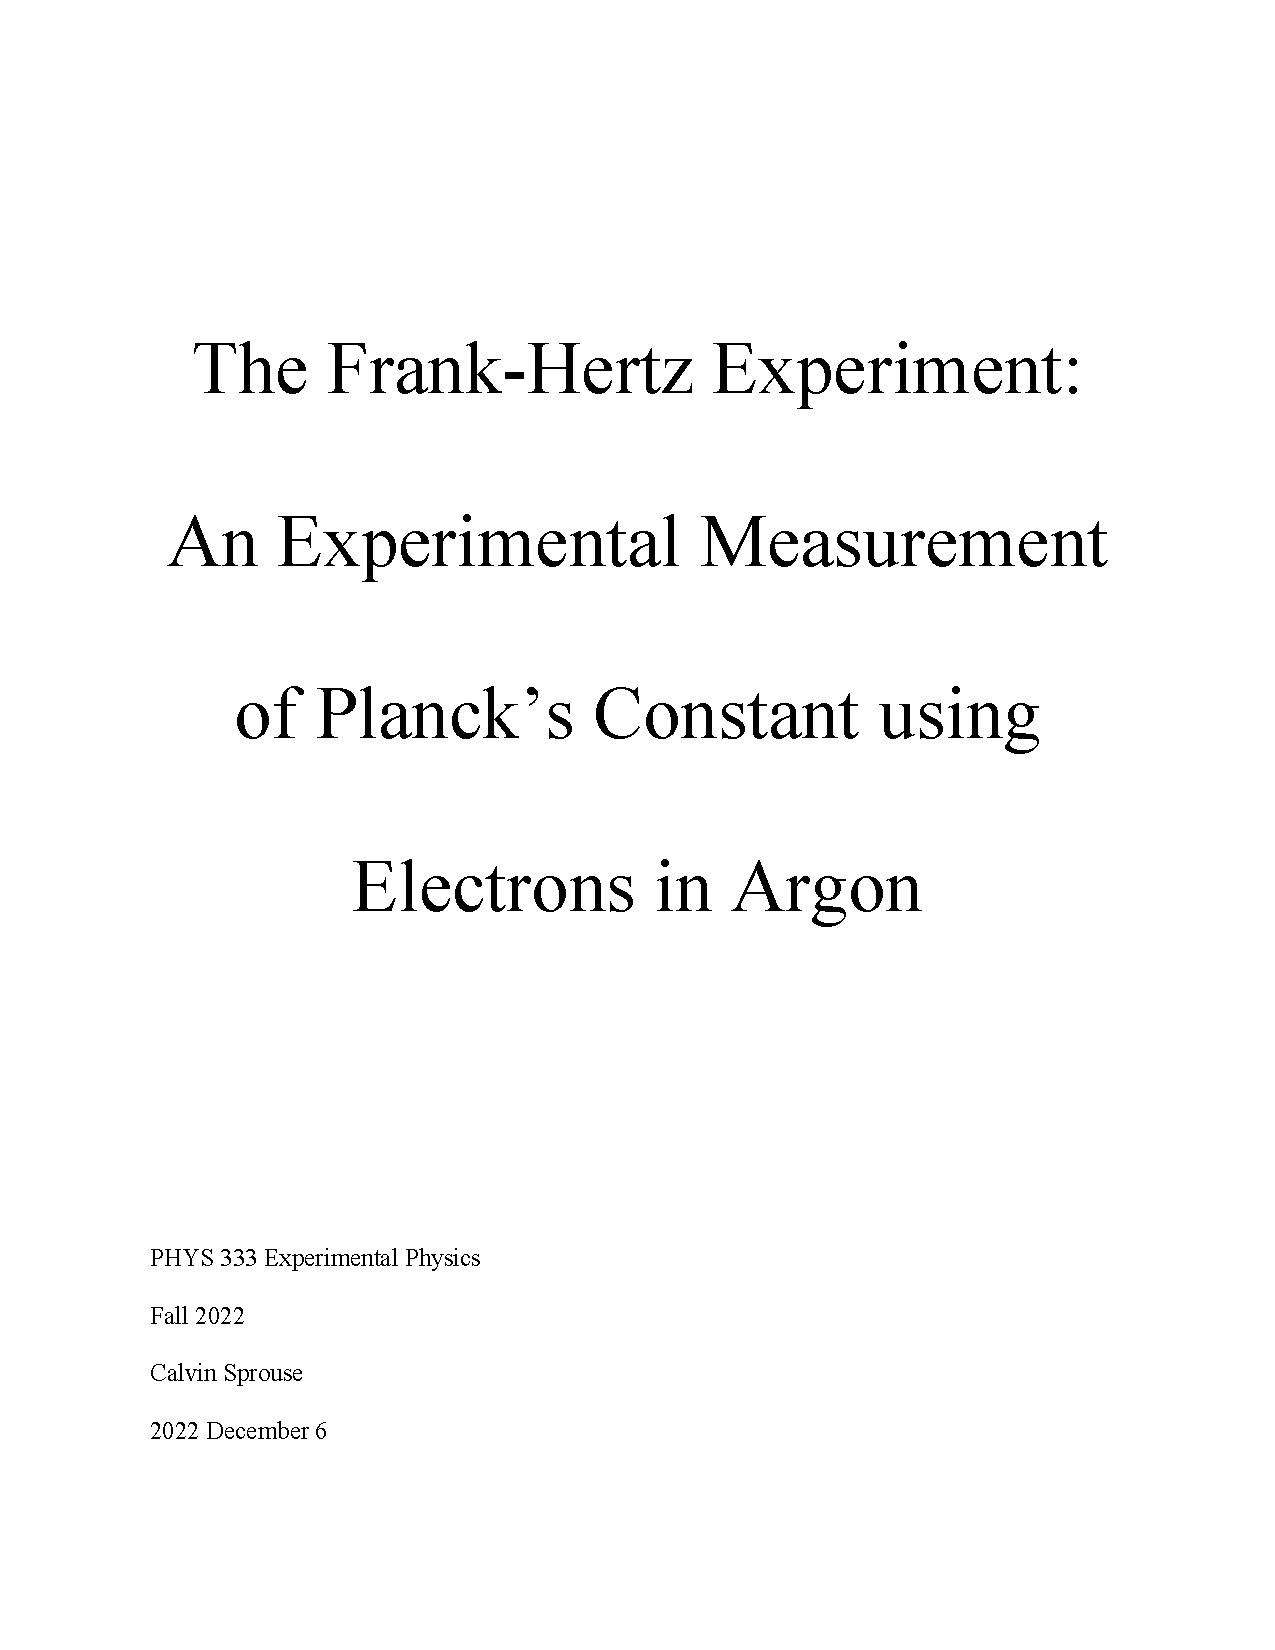
\includepdf[pages=-]{FullReportCalvinSprouse.pdf}
\end{document}
